%We report on our experience of applying the proposed design and implementation
%to the mechanization of language metatheories.

%To demonstrate the applicability of our design and implementation, we
%conduct two case studies.


\noindentparagraph{Type safety of STLCs.}

The first case study is the mechanization of the type safety theorem of
STLC and those of its extensions,
which has been occurring in the examples in this paper.
The code base is ported from Software Foundations~\cite{sf-pl}.
%
The base STLC family consists of about 400~LOC.
Lines of code in each of the four derived families
($\mathrm{Y}$, $\times$, $+$, and $\mu$ in the Venn diagram)
vary from 100 to 250, largely depending on how many constructors they
add to the inductive types.
%
The linguistic nature of our approach allows us to retain a programming
style similar to the original proofs in Software Foundations.

\begingroup
\small
\renewcommand*{\arraystretch}{0.75}

\def\CircFix{(135:0.707cm) circle (1.5cm)}
\def\CircProd{(45:0.707cm) circle (1.5cm)}
\def\CircIsorec{(-45:0.707cm) circle (1.5cm)}
\def\CircSum{(-135:0.707cm) circle (1.5cm)}

\definecolor{FixColor}{HTML}{FF9966}
\definecolor{ProdColor}{HTML}{66CCFF}
\definecolor{SumColor}{HTML}{FFFF66}
\definecolor{IsorecColor}{HTML}{FF6699}

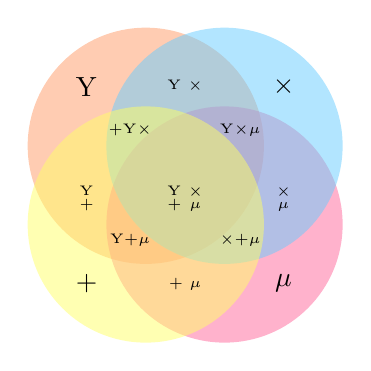
\begin{tikzpicture}
    \begin{scope}[shift={(0cm,-0cm)}, fill opacity=0.50]
        \fill[FixColor] \CircFix;
        \fill[IsorecColor] \CircIsorec;
        \fill[ProdColor] \CircProd;
        \fill[SumColor] \CircSum;
%       \draw \CircFix;
%       \draw \CircIsorec;
%       \draw \CircProd;
%       \draw \CircSum;
    \end{scope}

    \node at (0: 0) {%
        \begin{minipage}{1cm}\tiny
        \[\begin{array}{@{}c@{\ }c@{}}
            \mathrm{Y} & \times\\ + & \mu
        \end{array}\]
        \end{minipage}
    };
    \node at (-180: 1.25cm) {%
        \begin{minipage}{1cm}\tiny
        \[\begin{array}{@{}c@{}}
            \mathrm{Y}\\ +
        \end{array}\]
        \end{minipage}
    };
    \node at (0: 1.25cm) {%
        \begin{minipage}{1cm}\tiny
        \[\begin{array}{@{}c@{}}
            \times\\ \mu
        \end{array}\]
        \end{minipage}
    };
    \node at (90: 1.26cm) {\tiny$\mathrm{Y}\ \times$};
    \node at (-90: 1.26cm) {\tiny$+\ \mu$};
    \node at (135: 1.768cm) {$\mathrm{Y}$};
    \node at (-135: 1.768cm) {$+$};
    \node at (45: 1.768cm) {$\times$};
    \node at (-45: 1.768cm) {$\mu$};
    \node at (45: 0.988cm) {\tiny$\mathrm{Y}$$\times$$\mu$};
    \node at (-45: 0.988cm) {\tiny$\times$$+$$\mu$};
    \node at (-135: 0.988cm) {\tiny$\mathrm{Y}$$+$$\mu$};
    \node at (135: 0.988cm) {\tiny$+$$\mathrm{Y}$$\times$};

\end{tikzpicture}
\endgroup

Using individual families to organize the mechanization of individual
language features leads to a modular design that also facilitates code reuse.
%
Individually developed features can be easily composed (as mixins) to
form new STLC variants.

Composing features can lead to \emph{feature interactions}~\cite{batory2011feature}:
features working correctly in isolation may require coordination when composed.
For example, composing \lsti{STLCIsorec} and \lsti{STLCProd}
(\cref{fig:stlc-isorec-prod}) creates a need to extend \lsti{tysubst} to
handle \lsti{ty_prod}, which the type-checker enforces.

Elimination of inductive types defined via \lsti{FInductive} is
mostly via the \lsti{FRecursion} and \lsti{FInduction} commands.
An exception is a handful of trivial ``inversion lemmas''.
For example, consider the lemma \lsti!\forall t, \neg step tm_true t!
stating that \lsti!tm_true! is irreducible.
If \lsti{step} were an ordinary inductive type, then it could be proved in Coq
simply by \lsti{intros t H; inversion H}.
But \lsti{step} is extensible. So one way to prove the lemma is
by \lsti{FInduction} on \lsti{step} and verifying that
a derived family does not accidentally make \lsti{tm_true} reducible.
%lemma still holds in derived families that add new constructors to \lsti{step}.
%
We observe that it is lighter-weight to use overriding (\cref{sec:override}) instead:
the programmer can specify that the proof of the lemma should be overridden
in any derived family that further binds \lsti{step},
and in return, they are permitted to treat \lsti{step} as an ordinary
inductive type in the proof and thus use \lsti{inversion} to prove it.
The plugin then automatically tries the same proof script in a derived
family to override the proof. Although proof scripts rather
than proof terms are reused, this practice seems justified
by the triviality of the lemmas and the terseness of the proof scripts.

The current plugin implementation does not yet support
mutually inductive types or mutual induction, which are
useful for modeling languages much more complex than STLCs.
However,
we believe generalizing our design to mutually inductive types does
not pose theoretical challenges.


\noindentparagraph{Abstract interpreters for imperative languages.}

Our second case study is a mechanization of abstract interpreters
for simple imperative languages.
In addition to the metatheories, this case study produces abstract
interpreters that are directly ready for program extraction in Coq.

The code is organized into four families.
A base family, \lsti{Imp}, defines the abstract syntax of a while-language
with pure expressions and impure statements, via \lsti{FInductive}.
The semantic is formulated as a functional interpreter like a CEK machine\cite{felleisen1986control}, parameterized by a fuel value,
via \lsti{FRecursion}.
It contains \textasciitilde 200~LOC.

A second family, \lsti{ImpGAI}, extends \lsti{Imp} and contains
\textasciitilde 550~LOC.
It exports a generic framework for deriving
abstract interpreters with partial correctness.
The soundness theorem of this generic abstract interpreter, \lsti{analyze},
is with respect to the interpreter, \lsti{eval}, inherited from \lsti{Imp}.
It states that the abstraction relation \lsti{RState} over a
concrete state~\lsti{S} and an abstract state~\lsti{absS} is preserved
by the analysis:

\begin{centered}
\begin{minipage}{.86\textwidth}
\begin{lstlisting}[basicstyle=\fontsize{8.25}{9}\ttfamily]
\forall stmt fuel S absS, RState S absS -> RState (eval fuel stmt S) (analyze fuel stmt absS)
\end{lstlisting}
\end{minipage}
\end{centered}

\begin{wrapfigure}[13]{r}{0.13\textwidth}
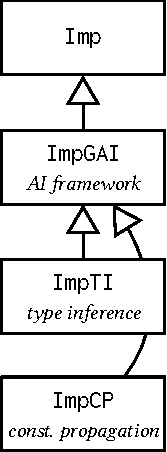
\includegraphics[scale=.68]{graphics/ai-casestudy.pdf}
\end{wrapfigure}

\noindent
\lsti{analyze} is defined via \lsti{FRecursion}, and the soundness theorem
is proved via \lsti{FInduction}.
This family leaves fields representing the abstract domain, the
abstraction relation, monotonicity of transfer functions, etc.\ 
largely unspecified or unproven\EDJ{It is not very relaxed. Currently everything is using a dicionary as memory model and stick with that. The abstract value for each expression is the one *really* unspecified.}---a derived family can instantiate these
``parameters'' by overriding appropriate fields (and also possibly extend the abstract syntax),
to create a sound, runnable abstract interpreter for a (possibly extended) while-language.

The other two families then extend \lsti{ImpGAI}.
Family \lsti{ImpTI} (\textasciitilde200~LOC) is an abstract
interpreter that does type inference~\cite{cousot1997types}.
Family \lsti{ImpCP} (\textasciitilde300~LOC) extends the abstract syntax
with natural number arithmetic,
and instantiates the generic abstract interpreter to perform constant propagation.

Our implementation of family polymorphism retains the computation
ability of the host proof assistant;
the two abstract interpreters in \lsti{ImpTI} and \lsti{ImpCP} are
directly ready for program extraction to OCaml and put them to test over queries.

We note that our plugin cannot yet allow the expression of two abstract
interpreters nested within the same family.
Work on nested inheritance~\cite{ncm2004,zm2017} points to a direction
to further increase the expressive power of our language design.

In addition to the two case studies above, we also use extensible
inductive types for modeling extensible context-free grammars and derive
decision procedures for them.

%\cref{sec:coqexample-stlc}
%\cref{sec:coqexample-analysis}
%\cref{sec:coqexample-parser}